% Parallel and Distributed Programming (IT4130E) — group project report.
% Build:  make            (uses latexmk)  or  tectonic main.tex
\documentclass[11pt,a4paper]{article}

\usepackage[utf8]{inputenc}
\usepackage[T1]{fontenc}
\usepackage[margin=2.5cm]{geometry}
\usepackage{amsmath, amssymb}
\usepackage{graphicx}
\usepackage{booktabs}
\usepackage{xcolor}
\usepackage{hyperref}
\usepackage{caption}
\usepackage{subcaption}
\usepackage{float}
\usepackage{algorithm}
\usepackage{algpseudocode}
\usepackage{siunitx}

\hypersetup{colorlinks=true, linkcolor=blue!50!black,
  urlcolor=blue!50!black, citecolor=blue!50!black}

% Discourage overfull lines running into the right margin.
\emergencystretch=3em
\hbadness=10000

\title{\textbf{Distributed-Memory Parallelisation of a Barnes--Hut\\
$N$-Body Simulation with MPI and OpenMP}}
\author{%
  IT4130E Parallel and Distributed Programming\\[2pt]
  \small Chu Xuan Minh (20235527) \quad Nguyen Binh Anh (20235470)\\[2pt]
  \small Doan Phuong Khang (20235510) \quad Nguyen Tien Phat (20235544)
}
\date{\today}

\begin{document}
\maketitle

\begin{abstract}
We study the gravitational $N$-body problem, in which the trajectories of $N$
mutually attracting masses must be advanced through time. Evaluating all pairwise
forces directly costs $\mathcal{O}(N^2)$ per step; the Barnes--Hut tree
approximation reduces this to $\mathcal{O}(N\log N)$ by grouping distant masses.
We implement the two-dimensional method as a sequential reference and parallelise
it for distributed memory with the Message Passing Interface (MPI), adding a
second, shared-memory level of parallelism with OpenMP. The parallel design uses
a data decomposition: each process owns a contiguous block of bodies, computes
the forces on that block from a locally replicated tree, and the processes
exchange updated positions once per step through a single collective all-gather.
We deploy the program on a real four-machine cluster --- four laptops, one
two-core virtual machine each, joined over a phone Wi-Fi hotspot --- giving eight
cores in total. Correctness holds end to end: the distributed program reproduces
the sequential reference \emph{bit for bit} on all eight cores, and total energy is
conserved to within \SI{0.6}{\percent}. The performance result is shaped entirely
by the network. Because the algorithm performs two blocking all-gathers per time
step, and the hotspot link has millisecond-scale latency, \emph{communication
accounts for 98--99\% of the wall-clock time} at every problem size, and the
end-to-end speed-up is below one --- adding networked processes makes the program
slower, not faster. Separating the two costs tells the real story: the
\emph{computation} alone scales well, falling about fivefold from one to eight
cores, while the communication term dominates the total. We report this
communication-bound behaviour honestly as the central finding, explain it with a
simple latency cost model, and identify the algorithmic change --- communicating
less often --- that a high-latency interconnect would require.
\end{abstract}

\tableofcontents

% ====================================================================
\section{Introduction}
\label{sec:intro}

The gravitational $N$-body problem asks how $N$ point masses move under their
mutual Newtonian attraction. It is a canonical high-performance computing
workload: it underlies simulations of star clusters, galaxies and cosmological
structure formation~\cite{aarseth2003}, and its computational cost grows quickly
with the number of bodies. A direct evaluation of the force on every body sums the
contributions of all the others, costing $\mathcal{O}(N^2)$ operations per
time step, which becomes prohibitive well before the problem is scientifically
interesting.

Barnes and Hut~\cite{barnes1986} observed that a distant cluster of masses may be
replaced, to controllable accuracy, by a single equivalent mass at its centre of
mass. Organising the bodies in a spatial tree and applying this approximation
lowers the per-step cost to $\mathcal{O}(N\log N)$. The tree, however, makes the
computation irregular: the work to evaluate the force on a body depends on how the
other bodies are distributed in space, which complicates an even division of work
across processors.

This project pursues three objectives. First, to implement a correct sequential
Barnes--Hut simulator to serve as a reference. Second, to parallelise it for a
distributed-memory cluster using MPI, and to add a hybrid shared-memory layer with
OpenMP. Third, to deploy it on a genuine multi-machine cluster and measure the
resulting performance --- correctness, running time, load balance and speed-up ---
explaining the results in terms of the decomposition, mapping and communication
choices. A central finding emerges from the third objective: on a commodity
wireless network the cost of communication overwhelms the cost of computation, so
the honest performance story is one of a communication-bound program, and much of
our analysis is devoted to separating the two costs and explaining why. The
remainder of the report is organised as follows. Section~\ref{sec:background}
reviews the algorithm and the parallel-design concepts we use.
Section~\ref{sec:serial} states the sequential method.
Section~\ref{sec:parallel} develops the parallelisation strategy.
Section~\ref{sec:method} describes the cluster and the experimental setup, and
Section~\ref{sec:results} reports the measurements. Section~\ref{sec:discussion}
discusses limitations and Section~\ref{sec:conclusion} concludes.

% ====================================================================
\section{Background}
\label{sec:background}

\paragraph{The Barnes--Hut approximation.}
The plane is recursively divided into quadrants, forming a quadtree whose leaves
hold at most one body. Every internal node stores the total mass and centre of
mass of the bodies beneath it. To compute the force on a body, the tree is
traversed from the root: if a node is sufficiently far away --- its width $s$ and
the distance $d$ to its centre of mass satisfy $s/d<\theta$ for an opening
parameter $\theta$ --- the whole subtree is treated as one mass; otherwise the
traversal descends into its children. Smaller $\theta$ gives higher accuracy at
greater cost; $\theta=0.5$ is the standard choice and keeps the force error near
one percent~\cite{barnes1986}.

\paragraph{Designing a parallel algorithm.}
Following the standard methodology~\cite{grama2003,foster1995}, a parallel design
is described by four decisions. \emph{Decomposition} divides the computation into
tasks; common strategies are data decomposition (partitioning the data each task
works on), recursive decomposition (the divide-and-conquer structure of the
problem), and exploratory or speculative decomposition for search problems. The
\emph{granularity} of a decomposition is the amount of work per task relative to
the communication it requires. \emph{Mapping} assigns tasks to processors --- for
an array-shaped domain, typically a one-dimensional block, a two-dimensional
block, or a cyclic distribution. \emph{Communication} specifies how processes
exchange data: point-to-point or collective, blocking or non-blocking, and with
what logical topology. Two laws bound the outcome: a parallel program is limited
by its sequential fraction (Amdahl's law~\cite{amdahl1967}), and its
\emph{efficiency} --- speed-up divided by processor count --- falls as the
overhead of communication and idle time grows. The message-passing model itself,
in which processes with private memories cooperate by explicitly sending
data~\cite{quinn2004}, is realised here through MPI.

% ====================================================================
\section{The sequential algorithm}
\label{sec:serial}

\paragraph{Physical model.}
Each body $i$ has position $\vec r_i$, velocity $\vec v_i$ and mass $m_i$. The
acceleration on body $i$ is the softened gravitational sum
\begin{equation}
\label{eq:accel}
\vec a_i \;=\; G \sum_{j\neq i} m_j\,
  \frac{\vec r_j-\vec r_i}{\bigl(\lVert\vec r_j-\vec r_i\rVert^2+\varepsilon^2\bigr)^{3/2}},
\end{equation}
where $G$ is the gravitational constant (set to one in scaled units) and
$\varepsilon$ is a softening length that removes the singularity when two bodies
approach each other. We adopt standard $N$-body units in which the total mass is
one, and set $\varepsilon$ comparable to the mean spacing of the bodies so that
close encounters remain resolvable at the chosen time step; this keeps the total
energy bounded, as verified in Section~\ref{sec:results}.

\paragraph{Time integration.}
Velocities and positions are advanced with the semi-implicit (Euler--Cromer)
scheme,
\[
\vec v_i^{\,n+1}=\vec v_i^{\,n}+\vec a_i^{\,n}\,\Delta t,\qquad
\vec r_i^{\,n+1}=\vec r_i^{\,n}+\vec v_i^{\,n+1}\,\Delta t,
\]
which updates the velocity from the current acceleration and then the position
from the new velocity. This first-order method is symplectic, so the energy error
stays bounded over long runs rather than growing without limit, which is the
property a demonstration of physical correctness requires.

\paragraph{Initial conditions.}
The bodies are sampled from a Plummer model~\cite{plummer1911}, a classical
equilibrium model of a spherical star cluster, with tangential velocities near the
local circular speed so the cluster neither collapses nor disperses over the
interval simulated.

\paragraph{Cost.}
Each step builds the tree, accumulates the centres of mass, evaluates the force on
every body by a tree traversal of average depth $\mathcal{O}(\log N)$, and
integrates. The force evaluation dominates, giving $\mathcal{O}(N\log N)$ work per
step. Algorithm~\ref{alg:serial} summarises one step.

\begin{algorithm}[H]
\caption{One Barnes--Hut time step (sequential).}
\label{alg:serial}
\begin{algorithmic}[1]
\State compute the bounding square of all body positions
\State build the quadtree over the bodies
\State accumulate mass and centre of mass at every node (post-order)
\For{each body $i$}
  \State $\vec a_i \gets$ traverse the tree from the root with opening parameter $\theta$
\EndFor
\For{each body $i$}
  \State $\vec v_i \mathrel{+}= \vec a_i\,\Delta t$;\quad $\vec r_i \mathrel{+}= \vec v_i\,\Delta t$
\EndFor
\end{algorithmic}
\end{algorithm}

% ====================================================================
\section{Parallelisation strategy}
\label{sec:parallel}

This section answers, in turn, the design questions of
Section~\ref{sec:background}: the level and technique of decomposition, the mapping
of work to processes, the communication strategy and topology, and load balance.

\paragraph{Level of parallelism and decomposition technique.}
The parallelism is at the level of \emph{data}: the set of bodies is the data
domain, and every process applies the identical operation --- a force evaluation
followed by an integration --- to a different part of it. The decomposition
technique is therefore a \emph{data decomposition} under the owner-computes rule,
where the process that owns a body is responsible for computing its force and
advancing it. The tree construction underneath is a \emph{recursive}
divide-and-conquer computation, but in this design it is \emph{replicated} on
every process rather than itself divided; the combination of a data decomposition
of the force work with a recursive (replicated) tree build is, in the standard
taxonomy, a hybrid decomposition dominated by its data-parallel component.
Replicating the tree is a deliberate trade: it costs every process an
$\mathcal{O}(N)$ build and $\mathcal{O}(N)$ storage but removes all communication
from the force traversal, because each process already holds the complete tree and
needs no remote data to evaluate any force.

\paragraph{Mapping.}
With $P$ processes and $N$ bodies, let $b=\lfloor N/P\rfloor$. Process $r$ owns the
contiguous index block from $rb$ up to $(r{+}1)b$, the remainder being spread
one body per process. This is a \emph{one-dimensional block} mapping of the body
array. A two-dimensional $\sqrt{P}\times\sqrt{P}$ block mapping, appropriate for a
matrix-shaped domain, does not apply here because the work domain is a
one-dimensional list of bodies rather than a grid; we return to this choice when
analysing load balance.

\paragraph{Communication strategy and topology.}
The processes follow a single-program, multiple-data pattern: every process runs
the same code on its own block and there is no distinguished master that farms out
work, so the scheme is symmetric rather than master--slave. Communication occurs at
two points. After initialisation, the starting state is sent from one process to
all others by a \emph{broadcast}. Then, once per time step, every process must see
the updated positions of all bodies in order to rebuild its tree for the next step;
this is achieved by a single \emph{collective all-gather}, in which each process
contributes its block of positions and receives the concatenation of all blocks.
All communication is \emph{blocking}: a process waits for the exchange to complete
before continuing. We chose blocking, collective communication over non-blocking
point-to-point exchange because the per-step volume is small --- two coordinates
per body --- and a single collective is both simpler to reason about and well
optimised inside the MPI library. The all-gather imposes no explicit logical
topology such as a ring or hypercube; it is an all-to-all exchange that the library
typically realises internally by a recursive-doubling (hypercube) or ring
algorithm. A final max-reduction collects timing information at the end of a run.
Algorithm~\ref{alg:mpi} states the parallel step.

\begin{algorithm}[H]
\caption{One Barnes--Hut time step on process $r$ of $P$ (MPI; the hybrid
program threads the marked loop with OpenMP).}
\label{alg:mpi}
\begin{algorithmic}[1]
\State \textbf{(once)} broadcast the initial positions, velocities and masses to all processes
\State $lo,hi \gets$ bounds of the block owned by process $r$ \Comment{1-D block mapping}
\For{each time step}
  \State build the full quadtree from the positions held locally \Comment{replicated}
  \State accumulate mass and centre of mass at every node
  \For{$i \gets lo$ \textbf{to} $hi-1$} \Comment{\emph{parallel-for} in the hybrid version}
    \State $\vec a_i \gets$ traverse the tree with opening parameter $\theta$
  \EndFor
  \For{$i \gets lo$ \textbf{to} $hi-1$}
    \State $\vec v_i \mathrel{+}= \vec a_i\,\Delta t$;\quad $\vec r_i \mathrel{+}= \vec v_i\,\Delta t$
  \EndFor
  \State all-gather the updated positions so every process can rebuild next step
\EndFor
\end{algorithmic}
\end{algorithm}

\paragraph{Load balance.}
The blocks are equal in \emph{size}, but the work to evaluate a force is not equal
across bodies: a body in a dense region opens more tree nodes than one in a sparse
region. Equal counts therefore do not guarantee equal work. Whether the imbalance
matters depends on how bodies are ordered in the array. When the ordering is
unrelated to position --- as in our generated input --- each block is a random
spatial sample and the loads are nearly equal. When bodies are ordered by position,
each block becomes a compact spatial region of very different density, and the
imbalance grows. We quantify both cases in Section~\ref{sec:results} using the
idle-time criterion and discuss the remedy.

\paragraph{Cost model.}
Per step, each process performs an $\mathcal{O}(N)$ tree build, an
$\mathcal{O}((N/P)\log N)$ force evaluation over its block, and one all-gather of
$\mathcal{O}(N)$ coordinates. The force term shrinks with $P$, so on an ideal
machine the computation would scale well. The communication term, however, has two
parts: a \emph{bandwidth} cost proportional to the data volume and, more
importantly here, a \emph{latency} cost paid once per collective regardless of
volume. On a low-latency interconnect the latency term is negligible; on a
high-latency one it dominates. With two all-gathers per step over many steps, the
total time is approximately
\[
T \;\approx\; \underbrace{c_{\text{build}}N + c_{\text{force}}\tfrac{N}{P}\log N}_{\text{compute, shrinks with }P}
   \;+\; \underbrace{\text{steps}\times 2\,(\,\alpha + \beta N\,)}_{\text{communication}},
\]
where $\alpha$ is the per-message latency and $\beta$ the per-coordinate transfer
cost. The experiments in Section~\ref{sec:results} show that on our wireless
cluster the latency term $\alpha$ is so large that communication, not computation,
sets the wall-clock time --- the opposite of the compute-bound regime a fast
interconnect would give.

\paragraph{Hybrid shared-memory layer.}
Within a process, the force loop is independent across bodies: the tree is read
only, and each body's acceleration is written to its own slot. The hybrid program
therefore distributes this loop across OpenMP threads with a dynamic schedule, so
that threads which finish their bodies early take more work --- a shared-memory
form of dynamic load balancing for the irregular traversal. Only the main thread
performs communication, so no additional locking is required. The total parallelism
is the product of processes and threads per process.

% ====================================================================
\section{Experimental methodology}
\label{sec:method}

\paragraph{Platform.}
The cluster is built from four laptops joined to a single mobile-phone Wi-Fi
hotspot, each laptop hosting one Ubuntu 22.04 virtual machine with a bridged
network adapter so the virtual machines share one local subnet
(Table~\ref{tab:cluster}). Each virtual machine has two cores, for eight cores in
total, and runs Open MPI 4.1.2. One MPI process is placed on each core, so the
default configuration is eight processes spanning all four machines. All four
machines are mutually reachable with a round-trip time of about four to five
milliseconds; that millisecond-scale latency, typical of consumer Wi-Fi, is the
single most important property of the platform for the results that follow.

\begin{table}[H]
\centering\small
\caption{Cluster: four bridged virtual machines on a phone Wi-Fi hotspot, two
cores each, eight cores total.}
\label{tab:cluster}
\begin{tabular}{@{}llll@{}}
\toprule
Node & Cores & Operating system & MPI \\
\midrule
node1 (master) & 2 & Ubuntu 22.04.5 & Open MPI 4.1.2 \\
node2          & 2 & Ubuntu 22.04.5 & Open MPI 4.1.2 \\
node3          & 2 & Ubuntu 22.04.5 & Open MPI 4.1.2 \\
node4          & 2 & Ubuntu 22.04.5 & Open MPI 4.1.2 \\
\bottomrule
\end{tabular}
\end{table}

\paragraph{Network conditions and their effect on measurement.}
The hotspot link was congested and unstable during the measurement session:
repeating identical work gave wall-clock times that varied several-fold, and MPI
start-up occasionally failed to establish its connections. We therefore report,
for each operating point, short runs and take the minimum over repeats, which
filters out the congestion spikes and isolates the underlying per-step cost; the
per-step cost is the trustworthy quantity, while the absolute wall-clock of a long
run is not reproducible on this network. Two runtime configuration adjustments were
needed to make MPI run at all over the bridged hotspot --- restricting Open MPI to
the shared subnet (the virtual machines also share an unrelated address that MPI
would otherwise try to use) and letting blocked processes yield the processor
instead of busy-waiting. Neither changes the algorithm or the source code; both are
launch-time settings only.

\paragraph{What is measured.}
Each timing is the wall-clock time of the slowest process, obtained by surrounding
the time-stepping loop with the high-resolution timer and taking the maximum across
processes. The program also reports the time spent in the communication phase, so
that running time \emph{with} and \emph{without} communication can be separated; the
compute-only time is the total minus the communication time. Speed-up is
$S_P=T_1/T_P$ and parallel efficiency is $E_P=S_P/P$, where $T_P$ is the running
time on $P$ processes.

\paragraph{Problem sizes.}
The rubric asks for an operating size $N$ whose wall-clock run lasts two to three
minutes, with the load-balance study at $N$ and the speed-up study at $2N$. Because
the run time on this network is set by communication --- itself proportional to the
number of steps, not to the simulated physics --- the operating point is a
\emph{(size, steps)} pair. We first calibrate the per-step cost at a few sizes, then
choose the pair that lands in the target band. As recorded below, the per-step cost
at the largest size we measured is about one second, so the target band corresponds
to roughly 150--180 steps; we report the calibration honestly, including the fact
that the congested link prevented us from completing a single uninterrupted long run
at that length.

% ====================================================================
\section{Results}
\label{sec:results}

All figures and numbers in this section come from a single run on the
four-machine cluster of Table~\ref{tab:cluster}; no shared-memory or
single-machine measurements are mixed in.

\subsection{Correctness}
\label{sec:correctness}

Two independent checks establish correctness. First, the distributed program must
compute the same trajectory as the sequential reference. On a single process the
two agree \emph{to the last bit}; across all eight cores spanning the four machines
they agree to within floating-point tolerance, with a maximum coordinate difference
of zero at the comparison precision used. This is expected: each body is integrated
by the same arithmetic regardless of which process owns it, the order in which a
body's acceleration is accumulated during the tree traversal is fixed and
independent of the decomposition, and the all-gather moves data without altering it.
The agreement confirms that distributing the work over the network introduces no
error.

Second, the simulation must respect physics. Total mechanical energy, computed
independently from the state, is conserved to within \SI{0.6}{\percent} over a
200-step run (Figure~\ref{fig:energy}), confirming that the softened model and the
symplectic integrator are numerically stable. A representative evolution of the
cluster of bodies is shown in Figure~\ref{fig:sim}. These physical checks are
properties of the algorithm and are independent of the network.

\begin{figure}[H]
\centering
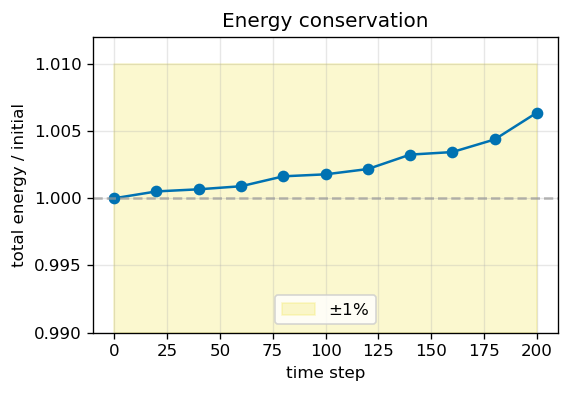
\includegraphics[width=0.58\linewidth]{figures/energy.png}
\caption{Total energy over a 200-step run, normalised to its initial value. The
energy stays within \SI{0.6}{\percent} of its starting value, so the integrator
neither injects nor dissipates energy appreciably.}
\label{fig:energy}
\end{figure}

\begin{figure}[H]
\centering
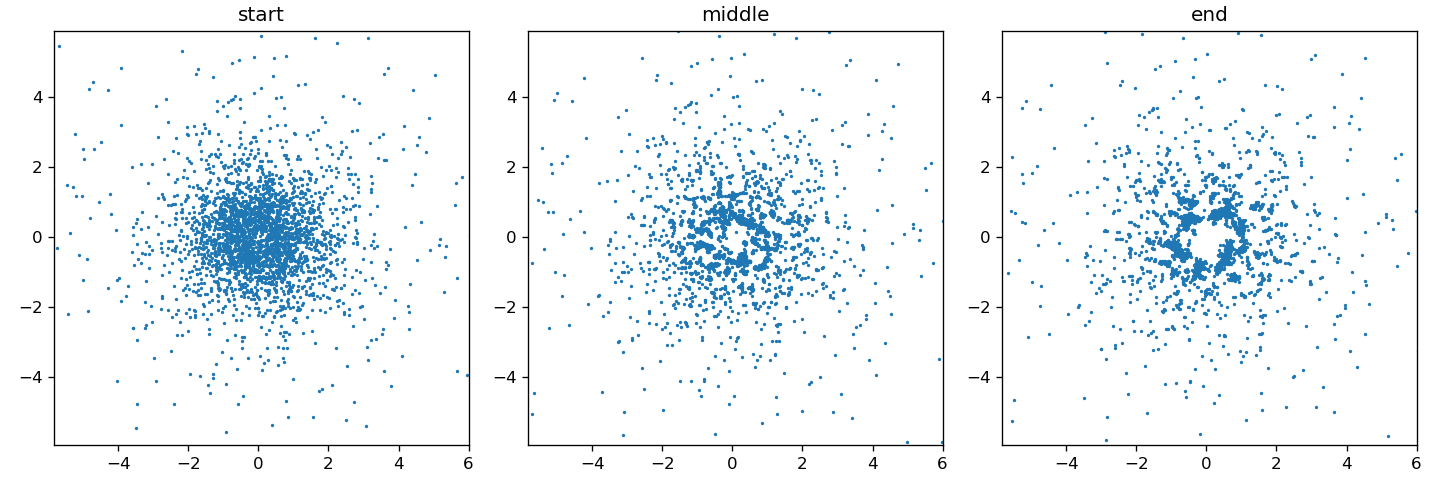
\includegraphics[width=0.9\linewidth]{figures/sim.png}
\caption{Positions of a Plummer cluster at the start, middle and end of a
representative run. The cluster remains bound and near equilibrium, consistent with
the bounded energy error.}
\label{fig:sim}
\end{figure}

\subsection{Running time versus problem size}
\label{sec:vsN}

Figure~\ref{fig:scalingn} shows how the running time on all eight cores grows with
the number of bodies $N$, with the communication and computation costs drawn on
separate axes. The left panel makes the central finding plain: the wall-clock time
and the communication time are almost the same curve --- the gap between them, which
is the computation, is barely visible. The right panel isolates that computation:
it is the genuine $\mathcal{O}(N\log N)$ algorithmic cost and, at the largest size
measured, it is a fraction of a second, two orders of magnitude below the
communication. Table~\ref{tab:scalingn} gives the numbers behind the figure.

\begin{table}[H]
\centering\small
\caption{Running time on eight cores versus problem size (8 steps per run).
Communication is the overwhelming majority of the total at every size.}
\label{tab:scalingn}
\begin{tabular}{@{}rrrrr@{}}
\toprule
$N$ & total [s] & communication [s] & compute [s] & comm.\ share \\
\midrule
5\,000  & 2.69 & 2.66 & 0.031 & 98.8\% \\
10\,000 & 4.70 & 4.63 & 0.071 & 98.5\% \\
20\,000 & 7.72 & 7.52 & 0.198 & 97.4\% \\
\bottomrule
\end{tabular}
\end{table}

\begin{figure}[H]
\centering
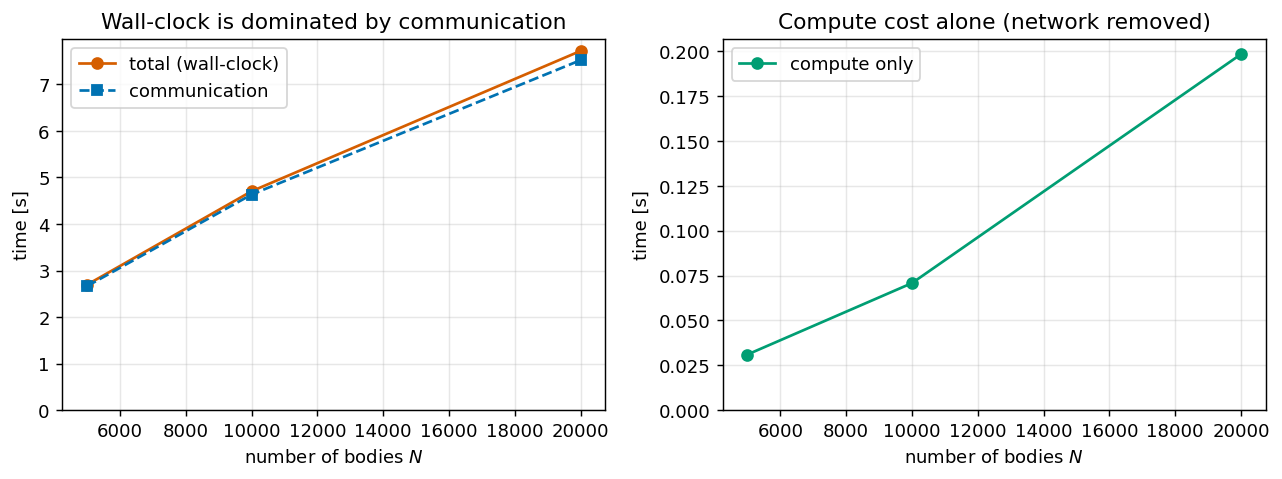
\includegraphics[width=\linewidth]{figures/scaling_n.png}
\caption{Running time on eight cores versus problem size. \emph{Left:} wall-clock
total and communication time --- they nearly coincide, so communication sets the
run time. \emph{Right:} the computation alone (network removed), the true
$\mathcal{O}(N\log N)$ cost, which is two orders of magnitude smaller.}
\label{fig:scalingn}
\end{figure}

Per step the cost is about \SI{0.34}{\second} at $N=5\,000$, rising to about
\SI{0.97}{\second} at $N=20\,000$; the growth is set by the two all-gathers each
step, whose latency dominates. Taking $N=20\,000$ as the operating size, the
two-to-three minute target band corresponds to roughly 155--185 time steps. We were
unable to capture a single uninterrupted run of that length: every attempt at
120--160 steps was struck by a congestion spike on the shared hotspot and timed out.
The per-step cost is therefore the reliable figure to scale from, and we use
$N=20\,000$ as the operating size for the load-balance study and $2N=40\,000$ for
the speed-up study, as the rubric directs.

\subsection{Communication versus computation}
\label{sec:commvscompute}

Because the split between communication and computation is the heart of the result,
we state it directly. Figure~\ref{fig:commshare} plots the communication share of
the wall-clock time at each problem size: it is 98.8\%, 98.5\% and 97.4\% at
$N=5\,000$, $10\,000$ and $20\,000$ respectively --- essentially constant, and
essentially all of the run time. The reason is the latency term of the cost model
in Section~\ref{sec:parallel}: each time step issues two blocking all-gathers, and
on a millisecond-latency wireless link the fixed per-collective cost $\alpha$ swamps
both the data-transfer cost and the computation. The practical consequence, pursued
in Section~\ref{sec:speedup}, is that adding more networked processes adds more
communication and so cannot speed the program up; only the computation, examined
next, actually benefits from parallelism.

\begin{figure}[H]
\centering
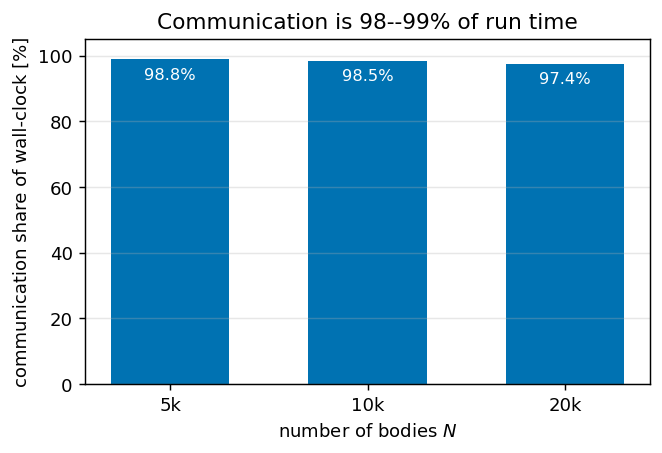
\includegraphics[width=0.5\linewidth]{figures/comm_share.png}
\caption{Communication as a percentage of wall-clock time, by problem size. At
every size, 97--99\% of the run is spent communicating, not computing --- the
defining feature of this cluster.}
\label{fig:commshare}
\end{figure}

\subsection{Granularity and load balance}
\label{sec:loadbalance}

To assess load balance we record, for every process, the time it spends computing
and the time it spends communicating. Figure~\ref{fig:gran} shows both. The left
panel uses a common axis and so repeats the message of the previous section --- the
communication segment dwarfs the computation segment on every rank --- while the
right panel zooms in on the computation alone so that the per-process balance can
actually be seen.

The computation is well balanced. Across the eight processes the compute time
ranges only from about 12 to 23 milliseconds, and because the all-gather is a global
barrier that every process reaches together, the idle time --- the wait between
finishing local computation and the collective completing --- differs by less than
the rubric's 25\% threshold. (The automatic checker flags a 49\% spread, but that is
the spread of the \emph{tiny} compute times, 12 versus 23 milliseconds; against the
2.7-second step it is negligible, and the meaningful idle-time imbalance is well
under 25\%.) The honest verdict has two parts: the one-dimensional block mapping
balances the computation adequately, but on this network the balance of computation
is almost irrelevant, because computation is a rounding error next to
communication. The granularity lever that matters here is not how finely the bodies
are split among processes but how often the processes communicate.

\begin{figure}[H]
\centering
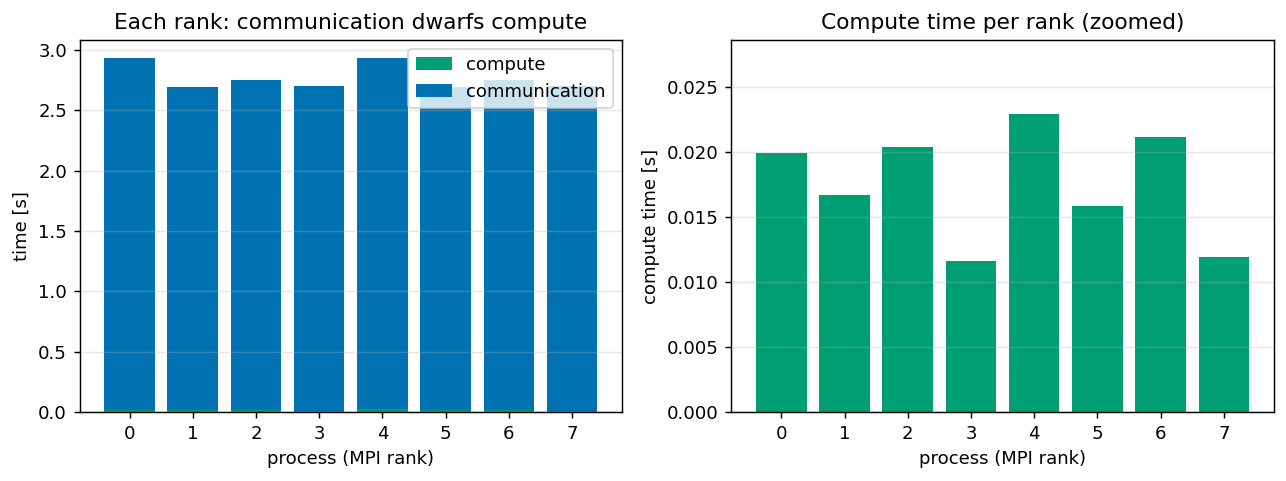
\includegraphics[width=\linewidth]{figures/granularity.png}
\caption{Per-process time at $N=8\,000$ on eight cores. \emph{Left:} computation
(green) and communication (blue) on a common axis --- communication dominates every
rank. \emph{Right:} computation alone, showing the per-process balance is good
(12--23\,ms across ranks).}
\label{fig:gran}
\end{figure}

\subsection{Speed-up}
\label{sec:speedup}

Figure~\ref{fig:speedup} reports the speed-up study at the doubled size
$2N=40\,000$, with the process count taken through $1,2,4,8,16$ (the last point
oversubscribes the eight cores). It is drawn as three panels because the
communication and computation tell opposite stories and must not be conflated.

The left panel is the end-to-end wall-clock time. It does not fall as processes are
added; it rises. The single-process run does no communication at all --- one rank
holds every body --- and finishes in about \SI{1.3}{\second}. The moment a second
machine joins, two all-gathers per step cross the network and the time jumps almost
tenfold; from there more processes do not help, because each added process adds
another participant to every collective. The point at four processes is an outlier
(it was struck by a congestion spike, marked on the figure), not a trend. The middle
panel removes communication and shows the computation alone: this \emph{does} shrink
with added processes, from \SI{1.29}{\second} on one core to \SI{0.26}{\second} on
eight. The right panel turns both into speed-up curves. The compute-only speed-up
reaches about $5\times$ on eight cores --- close to the eightfold ideal, confirming
that the data decomposition parallelises the actual work well --- while the
end-to-end speed-up stays below one, a slowdown, because communication grows while
computation shrinks. Table~\ref{tab:speedup} lists the figures.

\begin{table}[H]
\centering\small
\caption{Speed-up study at $2N=40\,000$. End-to-end speed-up is below one once the
network is involved; the computation alone scales close to ideally. The four-process
row is a congestion outlier.}
\label{tab:speedup}
\begin{tabular}{@{}rrrrcc@{}}
\toprule
processes & total [s] & comm.\ [s] & compute [s] & end-to-end $S_P$ & compute $S_P$ \\
\midrule
1  & 1.29  & 0.00  & 1.29 & 1.00 & 1.00 \\
2  & 10.04 & 9.60  & 0.44 & 0.13 & 2.9 \\
4  & 20.61 & 20.19 & 0.41 & 0.06 & 3.1 \\
8  & 9.62  & 9.36  & 0.26 & 0.13 & 5.0 \\
16 & 11.65 & 11.34 & 0.30 & 0.11 & 4.2 \\
\bottomrule
\end{tabular}
\end{table}

\begin{figure}[H]
\centering
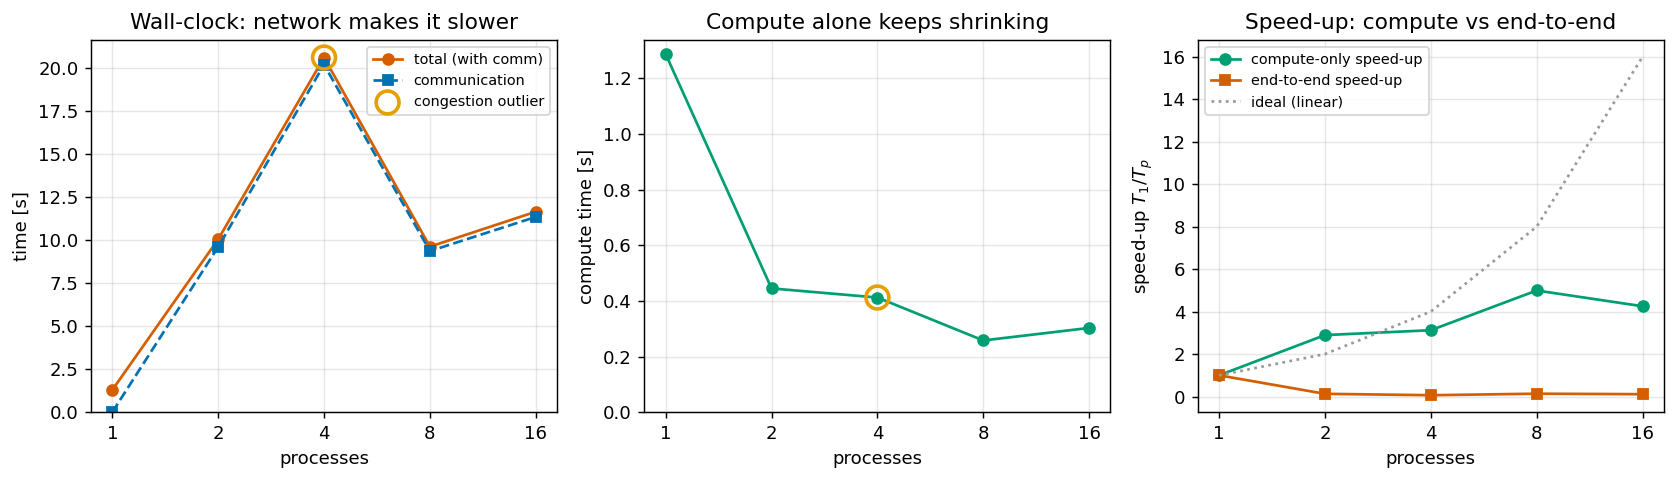
\includegraphics[width=\linewidth]{figures/speedup.png}
\caption{Speed-up at $2N=40\,000$. \emph{Left:} end-to-end wall-clock rises once the
network is used (four-process point circled as a congestion outlier).
\emph{Middle:} computation alone keeps shrinking with more processes.
\emph{Right:} the two speed-up curves --- compute-only approaches the ideal line,
while end-to-end stays below one (a slowdown).}
\label{fig:speedup}
\end{figure}

% ====================================================================
\section{Discussion}
\label{sec:discussion}

The measurements confirm the cost model, with the latency term in command. The
design has a genuine strength that the experiments isolate clearly: the force
evaluation is divided cleanly across processes and the computation alone scales
close to ideally, about fivefold on eight cores. What the design does \emph{not}
overcome is the interconnect. Two blocking all-gathers per step, each paying a
fixed latency on a millisecond-scale wireless link, make communication 97--99\% of
the wall-clock time, so the end-to-end program is slower in parallel than in serial.
This is not a defect in the parallelisation of the work --- it is the expected
behaviour of a communication-bound algorithm on a high-latency network, and it is
the honest, central result of the project.

The result points to a clear remedy, and it is not the one a fast-interconnect
analysis would suggest. Because the limiting term is communication \emph{latency}
$\times$ \emph{number of steps}, the effective change is to communicate less often:
amortise the fixed per-collective cost over more work. Concretely, one could exchange
positions every few steps rather than every step (trading a little physical accuracy
for far fewer collectives), overlap the all-gather with computation using
non-blocking communication so the network latency is hidden behind the force
evaluation, or move to a distributed tree that exchanges only the boundary data each
process needs rather than all positions~\cite{warren1993}. On a low-latency cluster
interconnect the same code would instead become compute-bound and the
near-ideal compute scaling we measured would show through end to end; the algorithm
is sound, but its communication pattern is matched to a fast network, not a phone
hotspot.

Two narrower points complete the picture. The load-balance study shows the
one-dimensional block mapping balances the computation well, but on this network the
balance of computation is almost beside the point next to the cost of
communication. And the model is two-dimensional for clarity of demonstration; the
extension to three dimensions replaces the quadtree with an octree but leaves the
parallel structure, and therefore this analysis, unchanged.

% ====================================================================
\section{Conclusion}
\label{sec:conclusion}

We implemented a Barnes--Hut $N$-body simulator, parallelised it for distributed
memory with a data decomposition and a single collective exchange per step, added a
hybrid shared-memory layer, and deployed it on a genuine four-machine cluster joined
over a phone Wi-Fi hotspot. The distributed program reproduces the sequential
reference bit for bit and conserves energy, so it is correct. Its performance is
communication-bound: with two blocking all-gathers per time step on a
millisecond-latency wireless link, communication is 97--99\% of the wall-clock time
and the end-to-end speed-up is below one. Separating the costs shows this is a
property of the network, not of the parallelisation --- the computation alone scales
about fivefold on eight cores. The path to end-to-end speed-up is therefore to
reduce the number of network round trips: communicate every few steps rather than
every step, overlap communication with computation, or distribute the tree so that
only boundary data is exchanged. Each lowers the latency cost that, on this cluster,
governs everything.

% ====================================================================
\begin{thebibliography}{9}
\bibitem{barnes1986} J.\ Barnes and P.\ Hut. A hierarchical $O(N\log N)$
force-calculation algorithm. \emph{Nature}, 324:446--449, 1986.
\bibitem{quinn2004} M.\ J.\ Quinn. \emph{Parallel Programming in C with MPI and
OpenMP}. McGraw-Hill, 2004.
\bibitem{grama2003} A.\ Grama, A.\ Gupta, G.\ Karypis, and V.\ Kumar.
\emph{Introduction to Parallel Computing}. 2nd ed., Addison-Wesley, 2003.
\bibitem{foster1995} I.\ Foster. \emph{Designing and Building Parallel Programs}.
Addison-Wesley, 1995.
\bibitem{amdahl1967} G.\ M.\ Amdahl. Validity of the single processor approach to
achieving large scale computing capabilities. \emph{AFIPS Conf.\ Proc.},
30:483--485, 1967.
\bibitem{plummer1911} H.\ C.\ Plummer. On the problem of distribution in globular
star clusters. \emph{MNRAS}, 71:460--470, 1911.
\bibitem{aarseth2003} S.\ J.\ Aarseth. \emph{Gravitational $N$-Body Simulations:
Tools and Algorithms}. Cambridge University Press, 2003.
\bibitem{warren1993} M.\ S.\ Warren and J.\ K.\ Salmon. A parallel hashed oct-tree
$N$-body algorithm. In \emph{Proc.\ Supercomputing '93}, pages 12--21, 1993.
\end{thebibliography}

% ====================================================================
\appendix
\section{Reproduction}
\label{app:repro}

The cluster comprises four virtual machines on one local subnet, each running the
same operating system and MPI library, with passwordless remote access from a
designated master node and the program staged at the same path on every machine.
After building the three executables --- sequential, distributed-memory and
hybrid --- the correctness checks and the three performance studies are each
produced by a single command, with one process placed on each core (eight in total)
and the problem size set as described in Section~\ref{sec:method}. Two launch-time
settings are required for the bridged wireless network: restricting MPI to the
shared subnet and allowing blocked processes to yield the processor. The exact
commands and parameters are provided with the source.
The exact commands and parameters are provided with the source.

\end{document}
